%
% File naaclhlt2018.tex

\documentclass[11pt,a4paper]{article}
\usepackage[hyperref]{naaclhlt2018}
\usepackage{times}
\usepackage{latexsym}
\usepackage{tikz}

\usepackage{url}

%\aclfinalcopy % Uncomment this line for the final submission
%\def\aclpaperid{***} %  Enter the acl Paper ID here

%\setlength\titlebox{5cm}
% You can expand the titlebox if you need extra space
% to show all the authors. Please do not make the titlebox
% smaller than 5cm (the original size); we will check this
% in the camera-ready version and ask you to change it back.

\title{Deep Multitask Learning for Transition-Based DAG Parsing}

\author{Daniel Hershcovich$^{1,2}$ \\
  \\\And
  Omri Abend$^2$ \\
  $^1$The Edmond and Lily Safra Center for Brain Sciences \\
  $^2$School of Computer Science and Engineering \\
  Hebrew University of Jerusalem \\
  \texttt{\{danielh,oabend,arir\}@cs.huji.ac.il}
  \\\And
  Ari Rappoport$^2$
}

\date{}

\begin{document}
\maketitle
\begin{abstract}
  Semantic representation schemes differ in many ways, but we show
  how they are similar and how this similarity can be exploited to
  improve parsing each of them.
  We train a general transition-based parser in a multitask setting
  and show improvements on multiple semantic parsing tasks.
\end{abstract}

\section{Introduction}\label{sec:introduction}

Following increased interest in semantic representation,
recent developments in natural language processing have focused on semantic parsing,
including frame-semantic parsing \cite{gildea2002automatic,swayamdipta2017frame,ringgaard2017sling},
Abstract Meaning Representation parsing \cite{damonte-17,11099},
Semantic Dependency Parsing \cite{P17-1186}, and
Universal Conceptual Cognitive Annotation parsing \cite{hershcovich2017a}, among others.
In parallel, Universal Dependency parsers \cite{dozat2016deep} are improving,
learning syntactic structure in a language-universal way.

While each of these representation schemes has its own set of distinctions it focuses on,
much of the semantic content is shared between many of them \cite{abend2017state}.
Given the success of multitask learning models in various tasks
\cite{collobert2008unified,luong2015multi,ruder2017overview}
including parsing specifically
\cite{Zhang2016StackpropagationIR,P17-1186,swayamdipta2017frame,guo2016exploiting}
and multilingual parsing \cite{TACL892},
we propose a multitask transition-based semantic parser.


\section{Tasks}\label{sec:tasks}

We consider four target representations in this work: UCCA, AMR, SDP and UD.

\subsection{Universal Conceptual Cognitive Annotation}\label{sec:ucca}

UCCA graphs are labeled, directed acyclic graphs (DAGs),
whose leaves correspond to the tokens of
the text. A node (or {\it unit}) corresponds to a terminal or
to several terminals (not necessarily contiguous) viewed as a
single entity according to semantic or cognitive considerations.
Edges bear a category, indicating the role of the sub-unit in the parent relation.

UCCA is a multi-layered representation, where each layer corresponds
to a ``module'' of semantic distinctions.
UCCA's \textit{foundational layer}, targeted in this paper, covers the predicate-argument
structure evoked by predicates of all grammatical categories
(verbal, nominal, adjectival and others), the inter-relations between them,
and other major linguistic phenomena such as coordination and multi-word expressions.
The layer's basic notion is the \textit{scene},
describing a state, action, movement or some other relation that evolves in time.
Each scene contains one main relation (marked as either a Process or a State),
as well as one or more Participants.
Further categories account for inter-scene relations and the internal structure of
complex arguments and relations (e.g. coordination, multi-word expressions and modification).

One incoming edge for each non-root node is marked as \textit{primary},
and the rest (mostly used for implicit relations and arguments) as \textit{remote} edges,
a distinction made by the annotator.
The primary edges thus form a tree structure, whereas the remote edges enable reentrancy,
forming a DAG.

\subsection{Abstract Meaning Representation}\label{sec:amr}

Abstract Meaning Representation \cite[AMR; ][]{banarescu2013abstract}
is a semantic representation for natural
language that embeds annotations related
to traditional tasks such as named entity
recognition, semantic role labeling, word
sense disambiguation and co-reference
resolution.

AMRs are rooted and directed
graphs with node and edge labels.
For most sentences in our dataset, the
AMR graph is a directed acyclic graph (DAG),
with a few specific cases where cycles are permitted.
These cases are rare, and for the purpose of
this paper, we consider AMR as DAGs.

\subsection{Semantic Dependency Parsing}\label{sec:sdp}

First defined in a SemEval 2014 shared task
\cite{oepen2014semeval}, and then extended by \citet{oepen2015semeval},
the broad-coverage semantic dependency parsing (SDP) task is centered around three
semantic formalisms whose annotations have been
converted into bilexical dependencies. The formalisms come
from varied linguistic traditions, but all three aim
to capture predicate-argument relations between
content-bearing words in a sentence.
While at first glance similar to syntactic dependencies,
semantic dependencies have distinct
goals and characteristics, more akin to semantic
role labeling \cite[SRL; ][]{gildea2002automatic} or
AMR. They abstract over different
syntactic realizations of the same or similar meaning.
Conversely, they attempt to distinguish
between different senses even when realized
in similar syntactic forms.
Structurally, they are labeled directed graphs
whose vertices are tokens in the sentence.
Their arc labels encode broadly-applicable semantic relations rather than being tailored
to any specific downstream application or
ontology.
They are not necessarily trees, because
a token may be an argument of more than one
predicate. Their analyses may optionally leave out non-content-bearing
tokens, such as punctuation or the infinitival ``to,'' or prepositions that simply mark
the type of relation holding between other words.
But when restricted to content-bearing tokens (including
adjectives, adverbs, etc.), the subgraph
is connected. In this sense, SDP provides a
whole-sentence analysis. This is in contrast to
PropBank-style SRL, which gives an analysis of
only verbal and nominal predicates \cite{Palmer:05}.
Semantic dependency graphs also tend to
have higher levels of nonprojectivity than syntactic
trees \cite{oepen2014semeval}. Sentences with
graphs containing cycles have been removed from
the dataset by the organizers, so all remaining
graphs are directed acyclic graphs.

We consider one of the three formalisms used in the SemEval shared task:
the DM (DELPH-IN MRS) representation, which comes
from DeepBank \cite{flickinger2012deepbank},
manually-corrected parses from the LinGO
English Resource Grammar \cite{copestake2000open}.
LinGO is a head-driven phrase
structure grammar \cite[HPSG; ][]{pollard1994head}
with minimal recursion semantics \cite{copestake2005minimal}.

\subsection{Universal Dependencies}\label{sec:ud}

In recent years, the Universal Dependencies
(UD) representation \cite{nivre2016universal} has become
the dominant dependency representation for
annotating treebanks in a large variety of languages.
The goal of the UD project is to provide
guidelines for cross-linguistically consistent treebank
annotations for as many languages as possible.



\section{Transition-Based Universal Parser}\label{sec:model}

Similarly to \citet{hershcovich2017a}, we use a transition-based parser
with a general transition system that allows parsing any DAG structure.
To demonstrate its applicability, we apply the parser to the four datasets
in a single-task setting.
The transition system supports reentrancies, discontinuities and non-terminal nodes.
In addition, we define a transition for labeling nodes, to support AMR parsing.

Transition-based parsers \cite{Nivre03anefficient} scan the text from start to end,
and create the parse incrementally by applying a \textit{transition}
at each step to the parser's state,
defined using three data structures: a buffer $B$ of tokens and nodes to be processed,
a stack $S$ of nodes currently being processed,
and a graph $G=(V,E,\ell)$ of constructed nodes and edges,
where $V$ is the set of \emph{nodes}, $E$ is the set of \emph{edges},
and $\ell : E \to L$ is the \emph{label} function, $L$ being the set of possible labels.
Some states are marked as \textit{terminal}, meaning that $G$ is the final output.
A classifier is used at each step to select the next transition based on features
encoding the parser's current state.
During training, an oracle creates training instances for the classifier,
based on gold-standard annotations.


\subsection{Transition Set.}
Given a sequence of tokens $w_1, \ldots, w_n$, we predict a graph $G$ over the sequence.
Parsing starts with a single node on the stack (an artificial root node), and the input tokens
in the buffer.

The transitions used in \citet{hershcovich2017a} are
the standard \textsc{Shift} and \textsc{Reduce} operations,
\textsc{Node$_X$} for creating a new non-terminal node and an $X$-labeled edge,
\textsc{Left-Edge$_X$} and \textsc{Right-Edge$_X$} to create a new primary $X$-labeled edge,
\textsc{Left-Remote$_X$} and \textsc{Right-Remote$_X$} to create a new remote $X$-labeled edge,
\textsc{Swap} to handle discontinuous nodes,
and \textsc{Finish} to mark the state as terminal.
In addition, we use a \textsc{Label$_i$} transition for $i=1,2$, adding a label for the $i$th
node from the top of the stack.
To keep the number of transitions manageable,
the node label itself is not part of the transition's identity,
instead being selected by a separate classifier.

\subsection{Classifier.}
Following \cite{hershcovich2017a}, we experiment with two different models for the parser:
a linear classifier with sparse features, trained with the averaged structured perceptron algorithm
\cite{Coll:04} and \textsc{MinUpdate} \cite{goldberg2011learning},
and a bidirectional LSTM with dense embedding features,
combined with a feedforward network.
We experiment with the softmax loss funnction and also softmax-margin
\cite{gimpel2010softmax}.

For all classifiers, inference is performed greedily,
and training is done with an oracle that provides a set of all possible labels at a given state
(but only valid transitions may be taken during training).
Hyperparameters are tuned on the development set for each task.

\begin{figure}[t]
	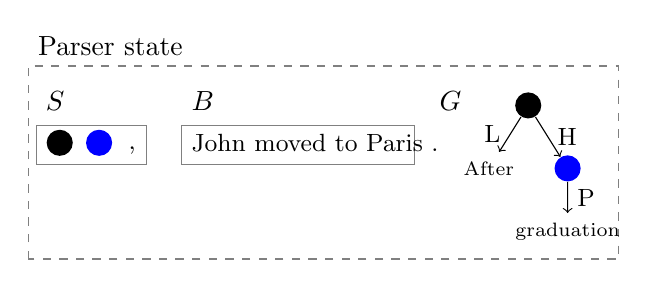
\begin{tikzpicture}[level distance=8mm, sibling distance=1cm]
	\node[anchor=west] at (0,1.5) {Parser state};
	\draw[color=gray,dashed] (0,-1.2) rectangle (7.5,1.25);
	\draw[color=gray] (.1,0) rectangle (1.5,.5);
	\node[anchor=west] at (.1,.8) {$S$};
	\node[fill=black, circle] at (.4,.275) {};
	\node[fill=blue, circle] at (.9,.275) {};
	\node[anchor=west] at (1.15,.175) {\small ,};
	\draw[color=gray] (1.95,0) rectangle (4.9,.5);
	\node[anchor=west] at (1.95,.8) {$B$};
	\node[anchor=west] at (1.95,.275) {\small John moved to Paris .};
	\node[anchor=west] at (5.1,.8) {$G$};
	\node[fill=black, circle] at (6.35,.75) {}
	  child {node  {\scriptsize After} edge from parent [->] node[left] {\small L}}
	  child {node [fill=blue, circle] {}
	  {
	    child {node {\scriptsize graduation} edge from parent [->] node[right] {\small P}}
	  } edge from parent [->] node[right] {\small H} };
	\end{tikzpicture}
	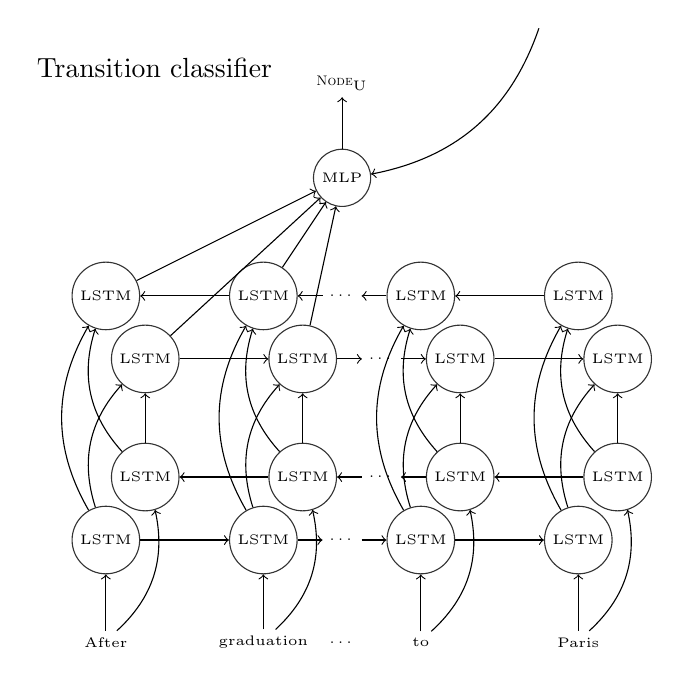
\begin{tikzpicture}[->]
	\node[anchor=west] at (0,6) {Transition classifier};
	\tiny
	\tikzstyle{main}=[circle, minimum size=7mm, draw=black!80, node distance=12mm]
	\foreach \i/\word in {1/{After},3/{graduation},5/{to},7/{Paris}} {
	    \node (x\i) at (\i,-1.3) {\word};
	    \node[main, fill=white!100] (h\i) at (\i,0) {LSTM};
        \path (x\i) edge (h\i);
	    \node[main, fill=white!100] (i\i) at (\i.5,.8) {LSTM};
        \path (x\i) edge [bend right] (i\i);
	    \node[main, fill=white!100] (l\i) at (\i.5,2.3) {LSTM};
        \path (h\i) edge [bend left] (l\i);
        \path (i\i) edge (l\i);
	    \node[main, fill=white!100] (k\i) at (\i,3.1) {LSTM};
        \path (i\i) edge [bend left] (k\i);
        \path (h\i) edge [bend left] (k\i);
	}
    \node (l4) at (4.5,2.3) {\ldots};
    \node (k4) at (4,3.1) {\ldots};
    \node (i4) at (4.5,.8) {\ldots};
    \node (h4) at (4,0) {\ldots};
    \node (x4) at (4,-1.3) {\ldots};
	\foreach \current/\next in {1/3,3/4,4/5,5/7} {
        \path (i\next) edge (i\current);
        \path (h\current) edge (h\next);
        \path (k\next) edge (k\current);
        \path (l\current) edge (l\next);
	}
    \node[main, fill=white!100] (mlp) at (4,4.6) {MLP};
	\foreach \i in {1,3} {
        \path (l\i) edge (mlp);
        \path (k\i) edge (mlp);
    }
    \coordinate (state) at (6.5,6.5);
    \path (state) edge [bend left] (mlp);
    \node (transition) at (4,5.8) {\textsc{Node}\textsubscript{U}};
    \path (mlp) edge (transition);
	\end{tikzpicture}
	\caption{Illustration of the model.
		Top: parser state (stack, buffer and intermediate graph).
		Bottom: BiLTSM architecture.
		Vector representation for the input tokens is computed
		by two layers of bidirectional LSTMs.
		The vectors for specific tokens are concatenated with
		embedding and numeric features from the parser state
		(for existing edge labels, number of children, etc.),
		and fed into the MLP for selecting the next transition.}
	\label{fig:model}
\end{figure}

We use the same features as \cite{hershcovich2017a}, and also node label features according to
previously predicted node labels for node in specific locations in the parser state.
We use sparse features for the linear classifier and embedding features for the BiLSTM.

POS tags and syntactic dependency labels are extracted using spaCy
\cite{honnibal-johnson:2015:EMNLP}.\footnote{\url{https://spacy.io}}
We use the categorical cross-entropy objective function and optimize the
NN classifiers with the Adam optimizer \cite{kingma2014adam}.
We use pretrained fastText word vectors \cite{bojanowski2016enriching} trained over Wikipedia.



\section{Multitask Transition-Based Parsing}\label{sec:multitask}

Since the same model can be applied to different tasks, we also train it jointly on multiple tasks.
Rather than sharing the whole set of parameters (and getting a mix of action labels as a result),
we share only part of the model.
Specifically, in addition to the task-specific input-encoding bidirectional LSTM,
we use a shared bidirectional LSTM. The outputs of both LSTMs are concatenated and
fed into the task-specific MLP.
This is similar to \citet{P17-1186}.




\section{Experiments}\label{sec:experiments}

We perform various experiments to evaluate which of the representation schemes benefit each other.
As a baseline, we train the parser separately on each task.

\subsection{Data}\label{sec:data}

For UCCA, we use the English Wikipedia corpus \cite{abend2013universal},
and in addition, the English, French and German 20K corpus \cite{sulem2015conceptual}.
For AMR, we use LDC2016E25 used in SemEval 2016 \cite{may2017semeval}.
For SDP, we use SemEval 2015 \cite{oepen2015semeval}.
For UD, we use UD v2 used in CoNLL 2017 \cite{silveira14gold,zeman2017conll}.
Table~\ref{tab:corpora} shows the size of each corpus.

\begin{table}
\begin{tabular}{lcc}
Corpus & \# Tokens & \# Sentences \\
\textbf{UCCA} \\
Wiki & 158433 & 5225 \\
20K Leagues en & 12339 & 506 \\
20K Leagues fr & 12929 & 547 \\
20K Leagues de & 113524 & 4764 \\
\textbf{UD} \\
English & 254850 & 16622 \\
French & 319253 & 16448 \\
German & 287110 & 15590 \\
\textbf{AMR} \\
LDC2016E25 & 708701 & 39260 \\
\textbf{SDP} \\
SemEval 2015 & 802717 & 35657 \\
\end{tabular}
\caption{Size of each corpus.\label{tab:corpora}}
\end{table}

\subsection{Results}\label{sec:results}

\subsection{Single-task}\label{sec:results_single}

The results for single-task parsing are shown in table~\ref{tab:single}.



\begin{table*}
\begin{tabular}{lccc|ccc}
\textbf{UCCA Wiki}
& \multicolumn{3}{c|}{Primary} & \multicolumn{3}{c}{Remote} \\
& \textbf{LP} & \textbf{LR} & \textbf{LF} & \textbf{LP} & \textbf{LR} & \textbf{LF} \\
\hline
Sparse & 63.4 & 64.3 & 63.8 & 17 & 14.3 & 15.5 \\
BiLSTM & 74.5 & 74.9 & 74.7 & 49.2 & 50.5 & 49.8 \\
\hline
\textbf{UD} & \multicolumn{3}{c|}{LAS} \\
& & & \textbf{F1} \\
Sparse & & & \\
BiLSTM & 77.4 & 77.4 & 77.4 \\
\hline
\textbf{AMR} & \multicolumn{3}{c|}{Smatch} \\
& \textbf{P} & \textbf{R} & \textbf{F1} \\
Sparse & 48.4 & 44.1 & 46.1 \\
BiLSTM & & & \\
\hline
\textbf{SDP} & \textbf{LP} & \textbf{LR} & \textbf{LF} \\
Sparse & & & \\
BiLSTM & & &
\end{tabular}
\caption{Single-task results on each dev set.\label{tab:single}}
\end{table*}

\subsection{Multitask}\label{sec:results_multi}

The results for multitask parsing are shown in table~\ref{tab:multi}.

\begin{table}
\begin{tabular}{lccc}
Parser \\
\textbf{UCCA} & Labeled Precision & Recall & F1 \\
\textbf{UD} & LAS F1 \\
\textbf{AMR} & Smatch Precision & Recall & F1 \\
\textbf{SDP} & Labeled Precision & Recall & F1 \\
\end{tabular}
\caption{Multitask results.\label{tab:multi}}
\end{table}



\section{Related work}\label{related_work}

In general, multitask learning involves optimizing more than one loss function \cite{ruder2017overview}.
However, in our case, the loss function has the same form across all tasks.
The same architecture and inference algorithm are applied to multiple annotation formats and datasets,
and only some of the parameters are shared between them: this is hard parameter sharing.



\bibliography{references}
\bibliographystyle{acl_natbib}

\end{document}
